%% LyX 2.2.1 created this file.  For more info, see http://www.lyx.org/.
%% Do not edit unless you really know what you are doing.
\documentclass[english,onecolumn]{IEEEtran}
\usepackage[T1]{fontenc}
\usepackage[latin9]{inputenc}
\usepackage{calc}
\usepackage{url}
\usepackage{amsmath}
\usepackage{amssymb}
\usepackage{graphicx}
\usepackage{babel}
\begin{document}

\title{Predictive Task Allocation}

\author{Saptarshi Bandyopadhyay}
\maketitle

\section{Motivation}

Predictive task allocation is the problem of assigning tasks to robotic
agents based on their state/capabilities and on the uncertain distribution
of future tasks. Predictive task allocation determines which robot
or group of robots will perform each task based on the robots\textquoteright{}
states (e.g., position, attitude, power-level) and capabilities (e.g.,
mobility, availability of appropriate sensor) and on the predicted
distribution of future tasks (e.g. the predicted location of future
areas of interest, or the likelihood that one of the robots will fail).
Predictive task allocation can be used both for closely coupled coordination
(e.g., deciding which robot takes what place in a formation) and for
loosely coupled coordination (e.g., which robot traverses to a new
spot to observe an interesting target).

The task allocation problem has long been of interest in the robotics
community. Proposed decentralized solution techniques include auction
algorithms, spatial partitioning algorithms, and Markov-chain based
algorithms; centralized team-forming and temporal partitioning algorithms
and centralized matching algorithms are also available. However, no
algorithm is available to solve the predictive task allocation problem
in a distributed manner for networks of heterogeneous agents (see
Table).

Here we aim to design a near-optimal centralized algorithm for the
predictive task allocation problem for the case where the probability
distribution of the events that trigger new tasks is known a priori.

\section{Problem Statement}

\subsection{Define variables}
\begin{itemize}
\item We state this problem in discrete time. Let $k$ represent the time
index, and $T$ is the total time. Therefore, $k\in\left\{ 1,\ldots,T\right\} $.
\item The number of agents at time $k$ is represented by $N_{k}$. Let
$i_{k}$ represent an agent index at time $k$, therefore $i_{k}\in\left\{ 1,\ldots,N_{k}\right\} $.
These are heterogeneous agents with heterogeneous capabilities. 
\item The number of tasks at time $k$ is represented by $M_{k}$. Let $j_{k}$
represent a task index at time $k$, therefore $j_{k}\in\left\{ 1,\ldots,M_{k}\right\} $.
Some of of these tasks are all-time tasks (e.g. patrolling) and some
are event-driven tasks (e.g. tracking an intruder).
\item Let $x_{i_{k},j_{k}}$ represent the indicator variable of agent $i_{k}$
doing task $j_{k}$, i.e., $x_{i_{k},j_{k}}=1$ if agent $i_{k}$
does task $j_{k}$ at time $k$ and $x_{i_{k},j_{k}}=0$ otherwise. 
\item Let $\mathcal{X}_{1:k-1}$ represent the list of all actions taken
by the agents from time $1,\ldots,k-1$, i.e., 
\begin{equation}
\mathcal{X}_{1:k-1}=\left\{ x_{i_{\tau},j_{\tau}},\forall\tau\in\{1,\ldots,k-1\},\forall i_{\tau}\in\left\{ 1,\ldots,N_{\tau}\right\} ,\forall j_{\tau}\in\left\{ 1,\ldots,M_{\tau}\right\} \right\} 
\end{equation}
\item Let the matrix $C_{k,\mathcal{X}_{1:k-1}}\in\mathbb{R}^{N_{k}\times M_{k}}$
represent the cost matrix at time $k$. The element $C_{k,\mathcal{X}_{1:k-1}}\left[i_{k},j_{k}\right]$
represents the value of doing task $j_{k}$ by agent $i_{k}$ at time
$k$, which depends on the past actions $\mathcal{X}_{1:k-1}$. It
can be composed of 2 terms: 
\begin{align}
C_{k,\mathcal{X}_{1:k-1}}\left[i_{k},j_{k}\right]= & \left(\textrm{Intrinsic value of doing the task }j_{k}\textrm{, which depends on }\mathcal{X}_{1:k-1}\right)\nonumber \\
 & \qquad\qquad-\left(\textrm{Effort incurred by agent }i_{k}\textrm{ to do the task }j_{k}\textrm{, which depends on }\mathcal{X}_{1:k-1}\right)\label{eq:define_C_k}
\end{align}
Here ``intrinsic value of doing the task $j_{k}$'' captures the
importance of the task, e.g., patrolling an area is significantly
lower importance than checking out an intruder, but patrolling an
area that hasn't been visited in some time is more valuable than patrolling
a recently visited area. ``Effort incurred by agent $i_{k}$ to do
the task $j_{k}$'' captures if an agent can do the task (if not,
then it is set to $\infty$) and how much effort does it need to expend,
e.g., tasks which need the agent to travel large distances should
cost more. 
\end{itemize}

\subsection{Additional comments about variables}

We now state some important aspects on tasks and costs:
\begin{itemize}
\item If the same task $j_{k}$ is present in time $k$ and time $k+1$,
and it was not done at time $k$, then ``intrinsic value of doing
the task $j_{k}$'' $\leq$ ``intrinsic value of doing the task
$j_{k+1}$'' (e.g., a region that hasn't been patrolled at time $k$
will have more intrinsic value at time $k+1$)
\item New tasks $j_{k}$ could get created at time $k$ with some known
probability distribution. (e.g., intruder could enter the controlled
space)
\item Doing task $j_{k}$ could trigger/create multiple task at time $k+1$.
(e.g., after checking out an intruder to be friendly or not-friendly,
different tasks are triggered)
\item Some un-done task from time $k$ could be destroyed at time $k+1$.
(e.g., intruder leaving the controlled space)
\item Agents could be created or destroyed at any time $k$ (e.g., agent
fails, or new agent is added)
\item The cost function $C_{k,\mathcal{X}_{1:k-1}}\left[i_{k},j_{k}\right]$
at time $k$ depends on $\mathcal{X}_{1:k-1}$, i.e., the previous
actions taken at times $1,\ldots,k-1$
\end{itemize}

\subsection{State Nonlinear Optimization Problem}

Finally, we are ready to state the predictive task allocation problem:

\noindent\fbox{\begin{minipage}[t]{1\columnwidth - 2\fboxsep - 2\fboxrule}%
\begin{align}
\underset{x_{i_{k},j_{k}\thinspace\forall i_{k},\forall j_{k},\forall k}}{\textrm{maximize}} & \sum_{k=1}^{T}\sum_{i_{k}=1}^{N_{k}}\sum_{j_{k}=1}^{M_{k}}C_{k,\mathcal{X}_{1:k-1}}\left[i_{k},j_{k}\right]x_{i_{k},j_{k}}\label{eq:maximize_net_value}\\
\textrm{subject to}\nonumber \\
 & \sum_{i_{k}=1}^{N_{k}}x_{i_{k},j_{k}}\leq1 &  & \forall j_{k}\in\left\{ 1,\ldots,M_{k}\right\} ,\forall k\in\left\{ 1,\ldots,T\right\} \label{eq:task_done_by_one_agent}\\
 & \sum_{j_{k}=1}^{M_{k}}x_{i_{k},j_{k}}\leq1 &  & \forall i_{k}\in\left\{ 1,\ldots,N_{k}\right\} ,\forall k\in\left\{ 1,\ldots,T\right\} \label{eq:agent_does_one_task}\\
 & x_{i_{k},j_{k}}\in\left\{ 0,1\right\}  &  & \forall i_{k}\in\left\{ 1,\ldots,N_{k}\right\} ,\forall j_{k}\in\left\{ 1,\ldots,M_{k}\right\} ,\forall k\in\left\{ 1,\ldots,T\right\} \label{eq:indicator_variable}
\end{align}
%
\end{minipage}}

\vspace{10pt}
\begin{itemize}
\item Eq. (\ref{eq:agent_does_one_task}) represents that an agent can do
only 1 task at a time step. (Is this need? Can an agent do all the
tasks at that location? For example, both patrolling and checking
out an intruder at the same location? In this case, we can collect
all the tasks at the same location and call it a combined task. But
capabilities of heterogeneous agents will come into play here when
we do the combining.)
\item Eq. (\ref{eq:task_done_by_one_agent}) represents that a task can
be done by only 1 agent at a time step. 
\end{itemize}

\section{Possible Simplifying Assumptions}

\subsection{Option 1: Assume $C_{k,\mathcal{X}_{1:k-1}}\rightarrow C_{k}$, i.e.,
remove the dependence on $\mathcal{X}_{1:k-1}$}

This will reduce the problem to a MILP. In my opinion, this is a bad
assumption because it removes the entire complexity of the problem
we are trying to address:
\begin{itemize}
\item In the definition $C_{k,\mathcal{X}_{1:k-1}}\left[i_{k},j_{k}\right]$
in Eq. (\ref{eq:define_C_k}), $\mathcal{X}_{1:k-1}$ ensures that
the intrinsic value of doing the task increases if it hasn't been
done in the previous time. 
\item $\mathcal{X}_{1:k-1}$ ensures that the effort incurred by agent $i_{k}$
to do the task $j_{k}$ depends on the current state of the agent.
e.g., tasks which need the agent to travel large distances should
cost more. This is necessary for the predictive part of the problem
statement. 
\end{itemize}

\subsection{Option 2: Simplistic Assumption on Tasks}

Let us assume that at the $k^{\textrm{th}}$ time instant, $M_{k}$
tasks are generated with some probability. The cost of doing a task
depends on the intrinsic value of doing the task $j_{k}$ (which does
NOT depend on $\mathcal{X}_{1:k-1}$) and on the agents current location
at the start of the $k^{\textrm{th}}$ time instant.

All the agents try to do some the tasks at this time instant. The
remaining undone tasks vanishes at the end of $k^{\textrm{th}}$ time
instant. 

We feel this problem captures the core essence of the original problem.
Here are the advantages of this assumption:
\begin{itemize}
\item We are ignoring deterministic tasks. We claim that they can be easily
added back. 
\item We are ignoring recurrent tasks (like patrolling), whose intrinsic
value depends on $\mathcal{X}_{1:k-1}$. Adding this back will be
difficult, but not impossible. 
\item This problem can be solved using Approximate DP. 
\end{itemize}
My main concern with Approximate DP is that we are losing the rigorousness
of the DP. How do we show our solution is good? 

\newpage

\section{Task Assignment for Homogeneous Agents to Tasks at One Time Step}

The state space is divided into $n_{\textrm{cell}}\in\mathbb{N}$
cells. 

There are $N$ agents at time step $t_{0}$. 

The cost of an agent to move from cell $i$ to cell $j$ is given
by $C[i,j]$, where $i,j\in\{1,\ldots,n_{\textrm{cell}}\}$. If an
agent cannot transition from cell $i$ to cell $j$, then $C[i,j]=\infty$.

There are M tasks at time step $t_{1}$. 

The reward incurred by an agent in cell $j$ is given by $R[j]$.
If there is no task in cell $j$, then $R[j]=0$.

\begin{figure}[h]
\begin{centering}
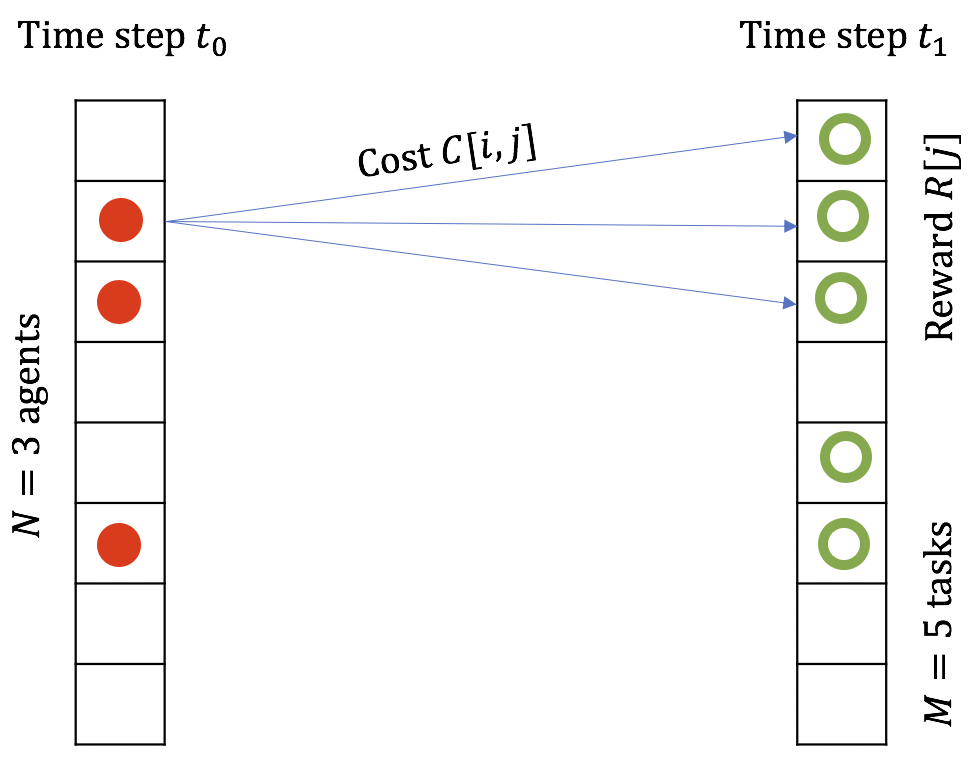
\includegraphics[width=5in]{simple_assignment}
\par\end{centering}
\caption{Simple Assignment Problem}
\end{figure}

Let $x[i,j]$ represent the indicator variable that an agent moves
from cell $i$ to cell $j$. 

Let $A[i]$ represent the indicator variable that an agent is present
in cell $i$ at time step $t_{0}$.

Our objective is the maximize the (reward - cost) gained by the agents. 

The assignment problem is given by the following ILP:

\noindent\fbox{\begin{minipage}[t]{1\columnwidth - 2\fboxsep - 2\fboxrule}%
\begin{align}
\underset{x[i,j],\thinspace\forall i,j\in\{1,\ldots,n_{\textrm{cell}}\}}{\textrm{maximize}} & \left(\sum_{j\in\{1,\ldots,n_{\textrm{cell}}\}}\left(R[j]\sum_{i\in\{1,\ldots,n_{\textrm{cell}}\}}x[i,j]\right)\right)\nonumber \\
 & \qquad\qquad-\left(\sum_{i\in\{1,\ldots,n_{\textrm{cell}}\}}\sum_{j\in\{1,\ldots,n_{\textrm{cell}}\}}C[i,j]\thinspace x[i,j]\right)\\
\textrm{subject to}\nonumber \\
 & x[i,j]\in\{0,1\} &  & \forall i,j\in\{1,\ldots,n_{\textrm{cell}}\}\label{eq:integer_condition}\\
 & \sum_{i\in\{1,\ldots,n_{\textrm{cell}}\}}x[i,j]\leq1 &  & \forall j\in\{1,\ldots,n_{\textrm{cell}}\}\label{eq:agent_in_one_cell}\\
 & \sum_{j\in\{1,\ldots,n_{\textrm{cell}}\}}x[i,j]=A[i] &  & \forall i\in\{1,\ldots,n_{\textrm{cell}}\}\label{eq:initial_conditions}
\end{align}
%
\end{minipage}}

Eq. (\ref{eq:agent_in_one_cell}) ensures that at most 1 agent can
be in any cell. 

Eq. (\ref{eq:initial_conditions}) ensures that initial conditions
are satisfied.

\newpage

We could also state this problem as a LP:

\noindent\fbox{\begin{minipage}[t]{1\columnwidth - 2\fboxsep - 2\fboxrule}%
\begin{align}
\underset{x[i,j],\thinspace\forall i,j\in\{1,\ldots,n_{\textrm{cell}}\}}{\textrm{maximize}} & \left(\sum_{j\in\{1,\ldots,n_{\textrm{cell}}\}}\left(R[j]\sum_{i\in\{1,\ldots,n_{\textrm{cell}}\}}x[i,j]\right)\right)\nonumber \\
 & \qquad\qquad-\left(\sum_{i\in\{1,\ldots,n_{\textrm{cell}}\}}\sum_{j\in\{1,\ldots,n_{\textrm{cell}}\}}C[i,j]\thinspace x[i,j]\right)\\
\textrm{subject to}\nonumber \\
 & x[i,j]\geq0 &  & \forall i,j\in\{1,\ldots,n_{\textrm{cell}}\}\label{eq:LP_cond_1}\\
 & x[i,j]\leq1 &  & \forall i,j\in\{1,\ldots,n_{\textrm{cell}}\}\label{eq:LP_cond_2}\\
 & \sum_{i\in\{1,\ldots,n_{\textrm{cell}}\}}x[i,j]\leq1 &  & \forall j\in\{1,\ldots,n_{\textrm{cell}}\}\\
 & \sum_{j\in\{1,\ldots,n_{\textrm{cell}}\}}x[i,j]=A[i] &  & \forall i\in\{1,\ldots,n_{\textrm{cell}}\}
\end{align}
%
\end{minipage}}

Eq. (\ref{eq:LP_cond_1}) and (\ref{eq:LP_cond_2}) convert the integer
constraint in Eq. (\ref{eq:integer_condition}) into linear constraints. 

The solution of this LP is the same as the above ILP. This can be
proved using Total Unimodularity.\footnote{Totally unimodular matrices give a quick way to verify that a linear
program is integral. \url{https://en.wikipedia.org/wiki/Unimodular_matrix#Total_unimodularity}}

\section{Task Assignment for Homogeneous Agents to Tasks in Multiple Time
Steps}

The state space is divided into $n_{\textrm{cell}}\in\mathbb{N}$
cells. 

There are $N$ agents at time step $t_{0}$. 

Let $t_{F}$ be the final time step for this lookahead policy. Hence
the time steps are $\{t_{0},t_{1},\ldots,t_{F}\}$.

The cost of an agent to move from cell $i$ in time step $t_{(k-1)}$
to cell $j$ in time step $t_{k}$ is given by $C_{k}[i,j]$, where
$i,j\in\{1,\ldots,n_{\textrm{cell}}\}$ and $k\in\{1,\ldots,F\}$.
If an agent cannot transition from cell $i$ in time step $t_{(k-1)}$
to cell $j$ in time step $t_{k}$, then $C_{k}[i,j]=\infty$.

There are $M_{k}$ tasks at time step $t_{k}$, where $k\in\{1,\ldots,F\}$. 

The reward incurred by an agent in cell $j$ in time step $t_{k}$
is given by $R_{k}[j]$. If there is no task in cell $j$ in time
step $t_{k}$, then $R_{k}[j]=0$.

The reward incurred by an agent in cell $j$ in time step $t_{F}$
is given by $R_{F}[j]$, where $R_{F}[j]$ is an approximation of
the future reward that the agent might get from that location.

\begin{figure}[h]
\begin{centering}
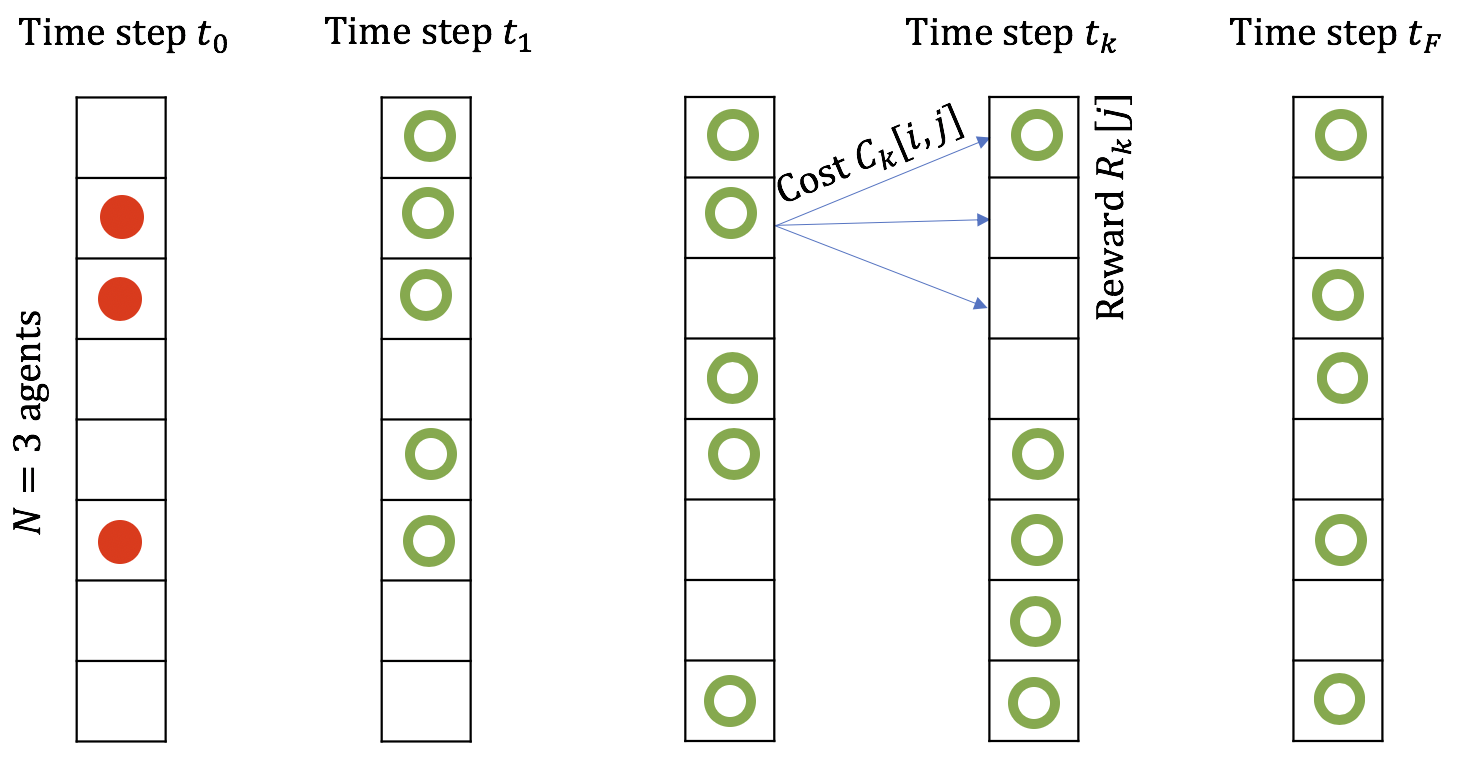
\includegraphics[width=6in]{multi_step_assignment}
\par\end{centering}
\caption{Multiple-Step Assignment Problem}
\end{figure}

Let $x_{k}[i,j]$ represent the indicator variable that an agent moves
from cell $i$ in time step $t_{(k-1)}$ to cell $j$ in time step
$t_{k}$. 

Let $A[i]$ represent the indicator variable that an agent is present
in cell $i$ at time step $t_{0}$.

Our objective is the maximize the (reward - cost) gained by the agents
over multiple time steps. 

The assignment problem is given by the following ILP:

\noindent\fbox{\begin{minipage}[t]{1\columnwidth - 2\fboxsep - 2\fboxrule}%
\begin{align}
\underset{\begin{array}{c}
x_{k}[i,j],\thinspace\forall i,j\in\{1,\ldots,n_{\textrm{cell}}\},\\
\forall k\in\{1,\ldots,F\}
\end{array}}{\textrm{maximize}} & \sum_{k\in\{1,\ldots F\}}\left(\left(\sum_{j\in\{1,\ldots,n_{\textrm{cell}}\}}\left(R_{k}[j]\sum_{i\in\{1,\ldots,n_{\textrm{cell}}\}}x_{k}[i,j]\right)\right)\right.\nonumber \\
 & \qquad\qquad-\left.\left(\sum_{i\in\{1,\ldots,n_{\textrm{cell}}\}}\sum_{j\in\{1,\ldots,n_{\textrm{cell}}\}}C_{k}[i,j]\thinspace x_{k}[i,j]\right)\right)
\end{align}
\begin{align}
\textrm{subject to}\nonumber \\
 & x_{k}[i,j]\in\{0,1\} &  & \forall i,j\in\{1,\ldots,n_{\textrm{cell}}\},\thinspace\forall k\in\{1,\ldots,F\}\label{eq:integer_condition-multi}\\
 & \sum_{i\in\{1,\ldots,n_{\textrm{cell}}\}}x_{k}[i,j]\leq1 &  & \forall j\in\{1,\ldots,n_{\textrm{cell}}\},\thinspace\forall k\in\{1,\ldots,F\}\label{eq:agent_in_one_cell-multi}\\
 & \sum_{j\in\{1,\ldots,n_{\textrm{cell}}\}}x_{1}[i,j]=A[i] &  & \forall i\in\{1,\ldots,n_{\textrm{cell}}\}\\
 & \sum_{i\in\{1,\ldots,n_{\textrm{cell}}\}}x_{k}[i,j]=\sum_{i\in n_{\textrm{cell}}}x_{k+1}[i,j] &  & \forall j\in\{1,\ldots,n_{\textrm{cell}}\},\thinspace\forall k\in\{1,\ldots,F-1\}\label{eq:flow_conservation}
\end{align}
%
\end{minipage}}

Eq. (\ref{eq:agent_in_one_cell-multi}) ensures that at most 1 agent
can be in any cell at any time step. 

Eq. (\ref{eq:flow_conservation}) ensures that equal number of agents
are entering and exiting a cell. This is used to conserve the number
of agents. 

\vspace{10pt}

We could also state this problem as a LP:

\noindent\fbox{\begin{minipage}[t]{1\columnwidth - 2\fboxsep - 2\fboxrule}%
\begin{align}
\underset{\begin{array}{c}
x_{k}[i,j],\thinspace\forall i,j\in\{1,\ldots,n_{\textrm{cell}}\},\\
\forall k\in\{1,\ldots,F\}
\end{array}}{\textrm{maximize}} & \sum_{k\in\{1,\ldots F\}}\left(\left(\sum_{j\in\{1,\ldots,n_{\textrm{cell}}\}}\left(R_{k}[j]\sum_{i\in\{1,\ldots,n_{\textrm{cell}}\}}x_{k}[i,j]\right)\right)\right.\nonumber \\
 & \qquad\qquad-\left.\left(\sum_{i\in\{1,\ldots,n_{\textrm{cell}}\}}\sum_{j\in\{1,\ldots,n_{\textrm{cell}}\}}C_{k}[i,j]\thinspace x_{k}[i,j]\right)\right)
\end{align}
\begin{align}
\textrm{subject to}\nonumber \\
 & x_{k}[i,j]\geq0 &  & \forall i,j\in\{1,\ldots,n_{\textrm{cell}}\},\thinspace\forall k\in\{1,\ldots,F\}\label{eq:LP_cond_1-multi}\\
 & x_{k}[i,j]\leq1 &  & \forall i,j\in\{1,\ldots,n_{\textrm{cell}}\},\thinspace\forall k\in\{1,\ldots,F\}\label{eq:LP_cond_2-multi}\\
 & \sum_{i\in\{1,\ldots,n_{\textrm{cell}}\}}x_{k}[i,j]\leq1 &  & \forall j\in\{1,\ldots,n_{\textrm{cell}}\},\thinspace\forall k\in\{1,\ldots,F\}\\
 & \sum_{j\in\{1,\ldots,n_{\textrm{cell}}\}}x_{1}[i,j]=A[i] &  & \forall i\in\{1,\ldots,n_{\textrm{cell}}\}\\
 & \sum_{i\in\{1,\ldots,n_{\textrm{cell}}\}}x_{k}[i,j]=\sum_{i\in n_{\textrm{cell}}}x_{k+1}[i,j] &  & \forall j\in\{1,\ldots,n_{\textrm{cell}}\},\thinspace\forall k\in\{1,\ldots,F-1\}
\end{align}
%
\end{minipage}}

Eq. (\ref{eq:LP_cond_1-multi}) and (\ref{eq:LP_cond_2-multi}) convert
the integer constraint in Eq. (\ref{eq:integer_condition-multi})
into linear constraints. 

We think the solution of this LP is the same as the above ILP.

Note that this formulation already accepts predictive tasks and deterministic
tasks. 

\section{Task Assignment for Heterogeneous Agents to Tasks in Multiple Time
Steps}

The state space is divided into $n_{\textrm{cell}}\in\mathbb{N}$
cells. 

There are $N$ heterogeneous agents at time step $t_{0}$. 

The agents are partitioned into $Q$ types, based on their capabilities. 

Let $t_{F}$ be the final time step for this lookahead policy. Hence
the time steps are $\{t_{0},t_{1},\ldots,t_{F}\}$.

The cost of an agent of type $q$ to move from cell $i$ in time step
$t_{(k-1)}$ to cell $j$ in time step $t_{k}$ is given by $C_{k}^{q}[i,j]$,
where $i,j\in\{1,\ldots,n_{\textrm{cell}}\}$ and $k\in\{1,\ldots,F\}$
and $q\in\{1,\ldots,Q\}$. If an agent of type $q$ cannot transition
from cell $i$ in time step $t_{(k-1)}$ to cell $j$ in time step
$t_{k}$, then $C_{k}^{q}[i,j]=\infty$.

There are $M_{k}$ tasks at time step $t_{k}$, where $k\in\{1,\ldots,F\}$. 

The reward incurred by an agent of type $q$ in cell $j$ in time
step $t_{k}$ is given by $R_{k}^{q}[j]$. If there is no task in
cell $j$ in time step $t_{k}$, then $R_{k}^{q}[j]=0$.

The reward incurred by an agent of type $q$ in cell $j$ in time
step $t_{F}$ is given by $R_{F}^{q}[j]$, where $R_{F}^{q}[j]$ is
an approximation of the future reward that the agent of type $q$
might get from that location.

\begin{figure}[h]
\begin{centering}
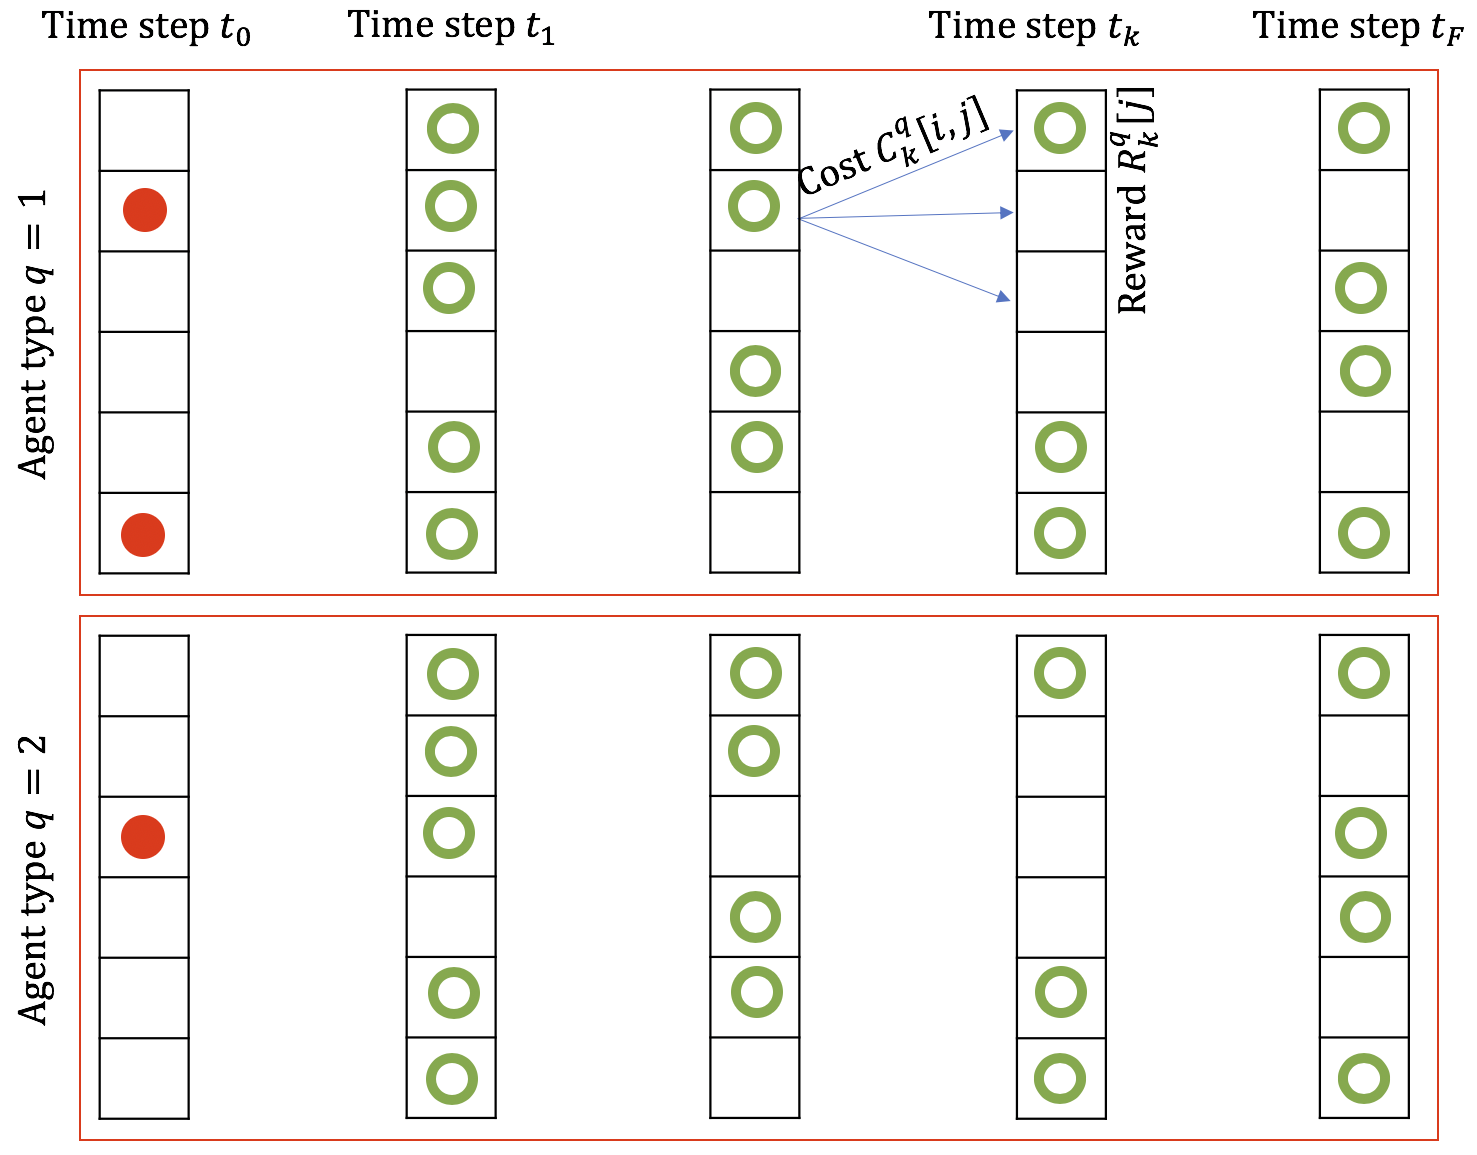
\includegraphics[width=6in]{heterogeneous_multi_step_assignment}
\par\end{centering}
\caption{Heterogeneous Multiple-Step Assignment Problem}
\end{figure}

Let $x_{k}^{q}[i,j]$ represent the indicator variable that an agent
of type $q$ moves from cell $i$ in time step $t_{(k-1)}$ to cell
$j$ in time step $t_{k}$. 

Let $A^{q}[i]$ represent the indicator variable that an agent of
type $q$ is present in cell $i$ at time step $t_{0}$.

Our objective is the maximize the (reward - cost) gained by the agents
over multiple time steps. 

The assignment problem is given by the following ILP:

\noindent\fbox{\begin{minipage}[t]{1\columnwidth - 2\fboxsep - 2\fboxrule}%
\begin{align}
\underset{\begin{array}{c}
x_{k}^{q}[i,j],\thinspace\forall i,j\in\{1,\ldots,n_{\textrm{cell}}\},\\
\forall k\in\{1,\ldots,F\},\thinspace q\in\{1,\ldots,Q\}
\end{array}}{\textrm{maximize}} & \sum_{k\in\{1,\ldots F\}}\left(\left(\sum_{j\in\{1,\ldots,n_{\textrm{cell}}\}}\left(\sum_{q\in\{1,\ldots,Q\}}\left(R_{k}^{q}[j]\sum_{i\in\{1,\ldots,n_{\textrm{cell}}\}}x_{k}^{q}[i,j]\right)\right)\right)\right.\nonumber \\
 & \qquad\qquad-\left.\left(\sum_{q\in\{1,\ldots,Q\}}\left(\sum_{i\in\{1,\ldots,n_{\textrm{cell}}\}}\sum_{j\in\{1,\ldots,n_{\textrm{cell}}\}}C_{k}^{q}[i,j]\thinspace x_{k}^{q}[i,j]\right)\right)\right)
\end{align}

\begin{align}
\textrm{subject to}\nonumber \\
 & x_{k}^{q}[i,j]\in\{0,1\} &  & \forall i,j\in\{1,\ldots,n_{\textrm{cell}}\},\thinspace\forall k\in\{1,\ldots,F\},\thinspace q\in\{1,\ldots,Q\}\label{eq:integer_condition-multi-hetero}\\
 & \sum_{q\in\{1,\ldots,Q\}}\sum_{i\in\{1,\ldots,n_{\textrm{cell}}\}}x_{k}^{q}[i,j]\leq1 &  & \forall j\in\{1,\ldots,n_{\textrm{cell}}\},\thinspace\forall k\in\{1,\ldots,F\}\label{eq:agent_in_one_cell-multi-hetero}\\
 & \sum_{j\in\{1,\ldots,n_{\textrm{cell}}\}}x_{1}^{q}[i,j]=A^{q}[i] &  & \forall i\in\{1,\ldots,n_{\textrm{cell}}\},\thinspace q\in\{1,\ldots,Q\}\\
 & \sum_{i\in\{1,\ldots,n_{\textrm{cell}}\}}x_{k}^{q}[i,j]=\sum_{i\in\{1,\ldots,n_{\textrm{cell}}\}}x_{k+1}^{q}[i,j] &  & \forall j\in\{1,\ldots,n_{\textrm{cell}}\},\thinspace\forall k\in\{1,\ldots,F-1\},\thinspace q\in\{1,\ldots,Q\}\label{eq:flow_conservation-hetero}
\end{align}
%
\end{minipage}}

Eq. (\ref{eq:agent_in_one_cell-multi-hetero}) ensures that at most
1 agent of any type can be in any cell at any time step. 

Eq. (\ref{eq:flow_conservation-hetero}) ensures that equal number
of agents of a given type are entering and exiting a cell. This is
used to conserve the number of agents. 

\vspace{10pt}

We could also state this problem as a LP:

\noindent\fbox{\begin{minipage}[t]{1\columnwidth - 2\fboxsep - 2\fboxrule}%
\begin{align}
\underset{\begin{array}{c}
x_{k}^{q}[i,j],\thinspace\forall i,j\in\{1,\ldots,n_{\textrm{cell}}\},\\
\forall k\in\{1,\ldots,F\},\thinspace q\in\{1,\ldots,Q\}
\end{array}}{\textrm{maximize}} & \sum_{k\in\{1,\ldots F\}}\left(\left(\sum_{j\in\{1,\ldots,n_{\textrm{cell}}\}}\left(\sum_{q\in\{1,\ldots,Q\}}\left(R_{k}^{q}[j]\sum_{i\in\{1,\ldots,n_{\textrm{cell}}\}}x_{k}^{q}[i,j]\right)\right)\right)\right.\nonumber \\
 & \qquad\qquad-\left.\left(\sum_{q\in\{1,\ldots,Q\}}\left(\sum_{i\in\{1,\ldots,n_{\textrm{cell}}\}}\sum_{j\in\{1,\ldots,n_{\textrm{cell}}\}}C_{k}^{q}[i,j]\thinspace x_{k}^{q}[i,j]\right)\right)\right)
\end{align}

\begin{align}
\textrm{subject to}\nonumber \\
 & x_{k}^{q}[i,j]\geq0 &  & \forall i,j\in\{1,\ldots,n_{\textrm{cell}}\},\thinspace\forall k\in\{1,\ldots,F\},\thinspace q\in\{1,\ldots,Q\}\label{eq:LP_cond_1-multi-hetero}\\
 & x_{k}^{q}[i,j]\leq1 &  & \forall i,j\in\{1,\ldots,n_{\textrm{cell}}\},\thinspace\forall k\in\{1,\ldots,F\},\thinspace q\in\{1,\ldots,Q\}\label{eq:LP_cond_2-multi-hetero}\\
 & \sum_{q\in\{1,\ldots,Q\}}\sum_{i\in\{1,\ldots,n_{\textrm{cell}}\}}x_{k}^{q}[i,j]\leq1 &  & \forall j\in\{1,\ldots,n_{\textrm{cell}}\},\thinspace\forall k\in\{1,\ldots,F\}\\
 & \sum_{j\in\{1,\ldots,n_{\textrm{cell}}\}}x_{1}^{q}[i,j]=A^{q}[i] &  & \forall i\in\{1,\ldots,n_{\textrm{cell}}\},\thinspace q\in\{1,\ldots,Q\}\\
 & \sum_{i\in\{1,\ldots,n_{\textrm{cell}}\}}x_{k}^{q}[i,j]=\sum_{i\in\{1,\ldots,n_{\textrm{cell}}\}}x_{k+1}^{q}[i,j] &  & \forall j\in\{1,\ldots,n_{\textrm{cell}}\},\thinspace\forall k\in\{1,\ldots,F-1\},\thinspace q\in\{1,\ldots,Q\}
\end{align}
%
\end{minipage}}

Eq. (\ref{eq:LP_cond_1-multi-hetero}) and (\ref{eq:LP_cond_2-multi-hetero})
convert the integer constraint in Eq. (\ref{eq:integer_condition-multi-hetero})
into linear constraints. 

We DONOT think the solution of this LP is the same as the above ILP,
because of the flow mixing in Eq. (\ref{eq:flow_conservation-hetero}).
But this fraction solution might be good enough since the tasks are
also probabilistic. 

Note that this formulation already accepts predictive tasks and deterministic
tasks. 
\end{document}
